
\begin{table}[!htb]
\centering
\caption{Statistics of dependency graphs generated for the 10 attacks}
\label{tab:stasticalSummary}
\resizebox{0.5\textwidth}{!}{
\begin{tabular}{crrrrr}
\hline
\textbf{Attack}        & \multicolumn{1}{c}{\textbf{CPR}} & \multicolumn{1}{c}{\textbf{ReadOnly}} & \multicolumn{1}{c}{\textbf{PrioTracker}} & \multicolumn{1}{c}{\textbf{NoDoze}} & \multicolumn{1}{c}{\textbf{Depprop}} \\ \hline
Wget Executable      & 363                              & 58                                    & 58                                       & 288                                 & 48                                   \\
Illegal Storage      & 62,073                           & 16,211                                & 6,948                                    & 10,260                              & 43                                   \\
Illegal Storage2     & 378,326                          & 89,779                                & 37,112                                   & 19,512                              & 7                                    \\
Hide File            & 3,273,769                        & 613,303                               & 114,614                                  & 37,253                              & 437                                  \\
Steal Information    & 3,291,208                        & 618,025                               & 115,223                                  & 20,426                              & 750                                  \\
Backdoor Download    & 60,390                           & 15,990                                & 6,024                                    & 269                                 & 20                                   \\
Annoying Server User & 318                              & 56                                    & 39                                       & 227                                 & 23                                   \\
Shellshcok           & 664                              & 243                                   & 179                                      & 491                                 & 34                                   \\
Dataleak             & 231                              & 87                                    & 67                                       & 120                                 & 14                                   \\
VPN Filter            & 1,118                            & 298                                   & 244                                      & 217                                 & 76                                   \\
Five Dir Case1       & 272                              & 18                                    & 18                                       & 75                                  & 7                                    \\
Five Dir Case3       & 78,075                           & 77,824                                & 7,496                                    & 598                                 & 33                                   \\
Theia Case1          & 816,277                          & 325,459                               & 176,800                                  & 17,057                              & 62                                   \\
Theia Case3          & 1,500,717                        & 537,424                               & 269,277                                  & 9,015                               & 10                                   \\
Trace Case5          & 971                              & 910                                   & 459                                      & 502                                 & 4                                    \\
\textbf{AVG}         & 630,984.80                       & 153,045.67                            & 48,970.53                                & 7,754.00                            & 104.53   \\ \hline                           
\end{tabular}
}
\end{table}



\subsection{RQ1: Revealing Attack Sequences}
\label{subsec:rq1}
To demonstrate the effectiveness of \tool in revealing the attack sequence by pruning non-critical edges, we compare \tool with 4 state-of-the-art techniques: CPR~\cite{reduction}, ReadOnly~\cite{loggc}, PrioTracker~\cite{liu2018priotracker}, and NoDoze~\cite{hassan2019nodoze}. 
%As discussed in \cref{subsubsec:entry-ranking},
\tool uses 6 entry nodes, composed of the top 2 entry nodes from the 3 types of system entities (\ie files, processes, and network connections), to perform forward causality analysis, which is shown to preserve all the critical edges (see \cref{subsec:rq2}).
CPR merges edges between two nodes if the time differences between the edges are within a threshold (\ie 10 seconds).
Readonly removes the edge whose source node is the read-only file. 
PrioTracker mainly uses the fanout of nodes to prioritize the dependencies in the causality analysis. 
We then adapt the computed priories as the dependency weights for edges and filter the edges with low weights.
%for comparison with \tool. 
NoDoze assigns an anomaly score for each edge based on the frequency of the corresponding system event, and then computes the anomaly score for each path. 
Paths having higher anomaly scores will be reported. 
We use the daily log file of the deployed system as the execution profile required by NoDoze and compute each path's anomaly score accordingly. 
Because we have the ground truth of each attack, we manually assign lower reputation scores for the malicious files and IP addresses as required by NoDoze.
Once NoDoze finishes computing the anomaly scores for the whole graph, we perform the graph reduction based on the anomaly score of each path in the dependency graph. 
Note that it is fairly easy for a technique to keep all the critical edges by keeping all the edges generated by the causality analysis from the POI event, but it is far more difficult to preserve the critical edges and filter the non-critical edges at the same time. 
Thus, we tune the parameters of all the techniques to preserve all the critical edges whenever possible, and compare the results of dependency graph reduction in terms of the number of edges.

\cref{tab:rq1} shows the dependency graph reduction of \tool and other approaches.
The results clearly show that \tool achieves the best performance for dependency graph reduction. 
On average, the size of the dependency graph generated by \tool (\ie the critical component output by \tool) is \emph{at least $33\times$ smaller than the second-best result} (\ie NoDoze) and three or four orders of magnitudes smaller than the other 3 methods.
We next explain the results comparison with each technique.

\tool is built upon CPR and thus the results demonstrate the better pruning power brought by the forward causality analysis from the top-ranked entry nodes.
Removing read-only files is heuristics-based and cannot robustly achieve good performance for different attacks as illustrated by the results (\eg $56$ for the ``Wget executable'' attack v.s. $600,000+$ for the ``Hide File'' attack).
The comparison with PrioTracker shows the superiority of our \textit{discriminative feature projection scheme} over the fanout feature in PrioTracker.

From the results, we can observe that NoDoze generally performs well but perform poorly for certain attacks, \eg the ``Hide File'' attack and the ``Steal information'' attack, whose dependency graphs have more than 3 million edges. 
The major reason is that there are many rare benign events in these dependency graphs that do not appear in the execution profiles used for training.
In NoDoze, the anomaly score of a given path is the product of each event's probability along the path. 
These rare benign events cause many paths that include these benign events to have higher anomaly scores, which greatly degrades the effectiveness of NoDoze.
In other words, the effectiveness of NoDoze heavily relies on whether the execution profile can capture all the benign events, which is generally difficult since the runtime environment of most organizations are quite versatile.
%
On the other hand, compared to NoDoze, \tool achieves better reduction results without sharing its two major limitations:
(1) \tool does not rely on third-party services to assign reputations for malicious files or IP addresses, which may introduce additional risks and complexity;
(2) \tool does not require the execution profile of the deployed system for training. 
These characteristics greatly reduce the difficulty of deploying \tool in a new system, enabling \tool to achieve better generalization than NoDoze.


\begin{figure}[t]
    \centering
    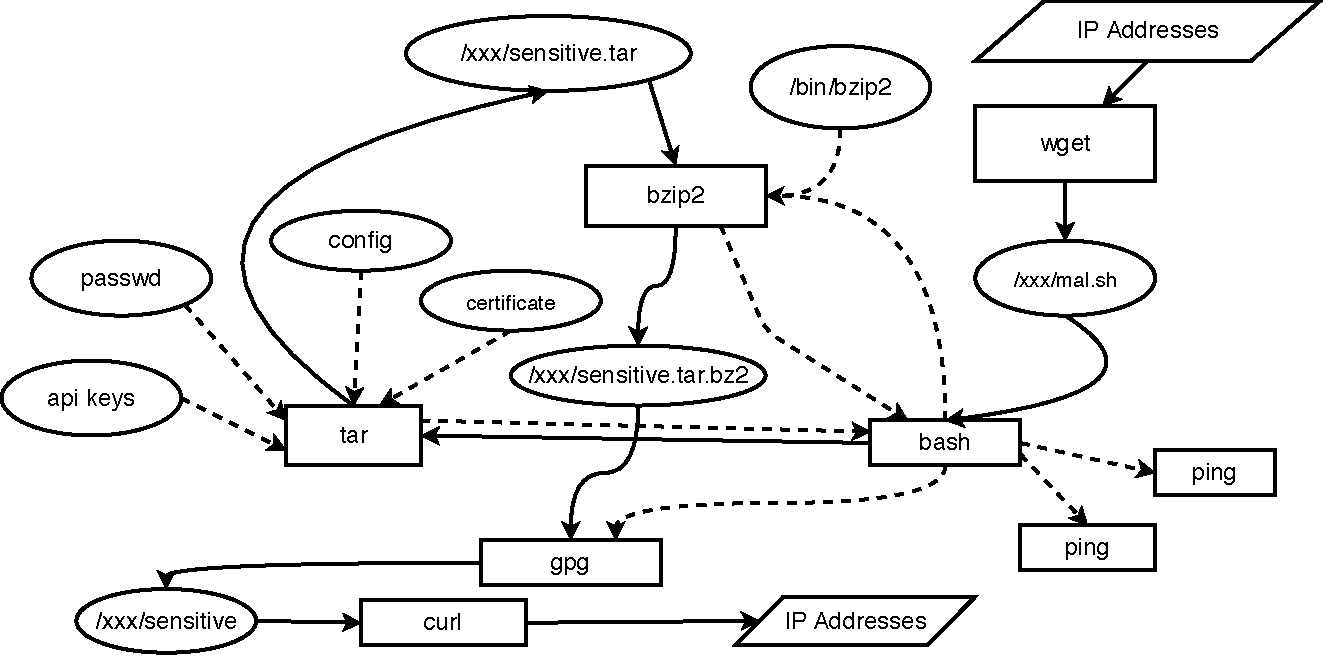
\includegraphics[width=0.47\textwidth]{figs/s&p/dataleak.pdf}
    \caption{Critical component (reduced dependency graph) generated by \tool for the ``Dataleak'' attack}
    \label{fig:dataleak}
\end{figure} 
\myparatight{Case Study}
\cref{fig:dataleak} shows the
%dependency graph 
critical component generated by \tool for the ``Dataleak'' attack. 
We use solid lines to represent the critical edges and dash lines to represent non-critical edges. 
From \cref{fig:dataleak}, we can observe that a malicious script \incode{mal.sh} is downloaded from a suspicious external IP address. 
This script starts a bash and then compresses the sensitive user data using \incode{tar}. 
After the compression, the attacker further compresses this file and encrypts it using \incode{bzip2} and \incode{gpg}. 
Then, the encrypted file is sent to the attacker host using \incode{curl}. 
For this attack, the attack sequence consists of 11 edges and \tool generates a graph of 24 edges that preserves all the 11 edges, while NoDoze generates 212 edges and the other techniques generates 31 edges at the best (\ie PrioTracker), demonstrating the superiority of \tool.






\eat{
Column \textit{NoDoze} shows the graph size processed by this method.


Column \emph{CPR} shows the graph size process by causality preserve reduction. 

Column \textit{Readonly} shows the graph size processed by this method.
Column \textit{Priotracker} shows the graph size processed by this method. 
Most of the existing works only focus on single characteristics of a given event, such as the source is read-only file or not, the frequency of a given event, or the fanout of dependency graph nodes. 
Compared with methods CPR, Readonly, Priotracker, and NoDoze, \tool uses more features to prioritize the important dependency relationships and most relevant entry points.
}



  